
disqus:

pagetime:

title: OI Wiki

\section{欢迎来到 \textbf{OI Wiki}。\href{https://github.com/24OI/OI-wiki}{\begin{figure}[h]
\centering
\includegraphics[width=0.5\textwidth]{https:/img.shields.io/github/watchers/24OI/OI-Wiki.svg?style=social&label=Watch} 
\caption{GitHub watchers}
\end{figure}} \href{https://github.com/24OI/OI-wiki}{\begin{figure}[h]
\centering
\includegraphics[width=0.5\textwidth]{https:/img.shields.io/github/stars/24OI/OI-Wiki.svg?style=social&label=Stars} 
\caption{GitHub stars}
\end{figure}}}

\href{https://github.com/24OI/OI-wiki}{\begin{figure}[h]
\centering
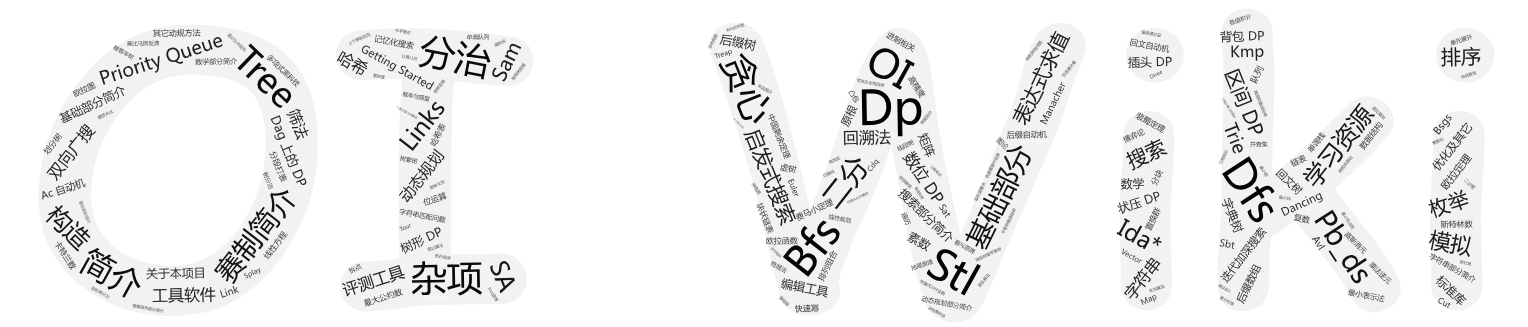
\includegraphics[width=0.5\textwidth]{images/wordArt.png} 
\caption{Word Art}
\end{figure}}

\textbf{OI} (Olympiad in Informatics,信息学奥林匹克竞赛)在中国起源于 1984 年,是五大高中学科竞赛之一。自 1989 年起,每年还会选拔出国家集训队选手准备 IOI (International Olympiad in Informatics,国际信息学奥林匹克竞赛)。

\textbf{ACM-ICPC} (ACM International Collegiate Programming Contest, ACM 国际大学生程序设计竞赛)由美国计算机协会(ACM)主办,由 ICPC 基金会负责组织,是最具影响力的大学生计算机竞赛。ICPC 主要分为区域赛(Regional)和总决赛(World Finals)两部分。

\textbf{OI Wiki} 致力于成为一个免费开放且持续更新的知识整合站点,大家可以在这里获取关于 \textbf{编程竞赛 (competitive programming)} 有趣又实用的知识,我们为大家准备了竞赛中的基础知识、常见题型、解题思路以及常用工具等内容,帮助大家更快速深入地学习编程竞赛。

本项目受 \href{https://ctf-wiki.github.io/ctf-wiki/}{CTF Wiki} 的启发,在编写过程中参考了诸多资料,在此一并致谢。

本项目文档内容托管在 \href{https://github.com/24OI/OI-wiki}{GitHub},主要使用 \href{https://github.com/24OI/OI-wiki/issues}{Issues} / \href{https://jq.qq.com/?_wv=1027&k=5EfkM6K}{QQ} / \href{https://t.me/OIwiki}{Telegram} / \href{https://discord.gg/xXdYSMq}{Discord} 进行交流沟通,期待你的加入。

Telegram 群组链接为 \href{https://t.me/OIwiki}{@OIwiki} , QQ 群号码为 \href{https://jq.qq.com/?_wv=1027&k=5EfkM6K}{\texttt{588793226}},欢迎加入。

\subsection{Material color palette 颜色主题}

\subsubsection{Primary colors 主色}

\begin{QUOTE}{}{}
默认 \texttt{white}
\end{QUOTE}

点击色块可更换主题的主色





\subsubsection{Accent colors 辅助色}

\begin{QUOTE}{}{}
默认 \texttt{red}
\end{QUOTE}

点击色块更换主题的辅助色




